\chapter{Postavitev sistema}
\section{Kaj potrebujemo}
\subsection{Hardware}
Za postavitev potrebujemo:
\begin{itemize}
    \item PC z operaciskim sistemom Windows (10),
    \item Raspberry Pi 3 Model B+,
    \item Raspberry Pi camera (HQ+objektiv),
    \item dve National Instruments analog output kartici (NI9263),
    \item National Instruments analog input kartica (IEPE) (NI 9234),
    \item laser + glava z zrcali.
\end{itemize}
\subsection{Software}
Od programske opreme se potrebuje:
\begin{itemize}
    \item \href{https://knowledge.ni.com/KnowledgeArticleDetails?id=kA03q000000YGQwCAO&l=sl-SI}{Ni MAX},
    \item python 3.9.
\end{itemize}
Python paketi uporabljeni v projektu:
\begin{itemize}
    \item numpy 1.21.0,
    \item matplotlib 3.4.2,
    \item scipy 1.7.0,
    \item openCV 4.5.2.54,
    \item nidaqmx 0.5.7,
    \item imagezmq 1.1.1,
    \item pyFRF 0.40,
    \item pyEMA 0.23,
    \item pyExSi 0.42.
\end{itemize}
Python skripte potrebne za delovanje programa:
\begin{itemize}
    \item gui.py,
    \item MSLK.py,
    \item RPi\_MSLK.py.
\end{itemize}

\section{Raspberry Pi}
Na RPi \href{https://www.raspberrypi.org/documentation/computers/getting-started.html}{naložimo operacijski sitem}. Nato odpremo \textit{Raspberry Pi Configuration} (slika \ref{fig:pi_nast}) ter spremenimo \textit{hostname}(v našem primeru v pi-kamera). Pod \textit{Interfaces} omogočimo Camera in SSH (da nastavitve začnejo delovati, je potreben reboot). V izbrano mapo kopiramo še skripto \href{https://github.com/nekajcasa/MSLK}{RPi\_MSLK.py} (v našem primeru je to desktop). Za delovanje je potrebno povezati RPi z ethernet kablom na PC.
\begin{figure}[H]
    \centering
    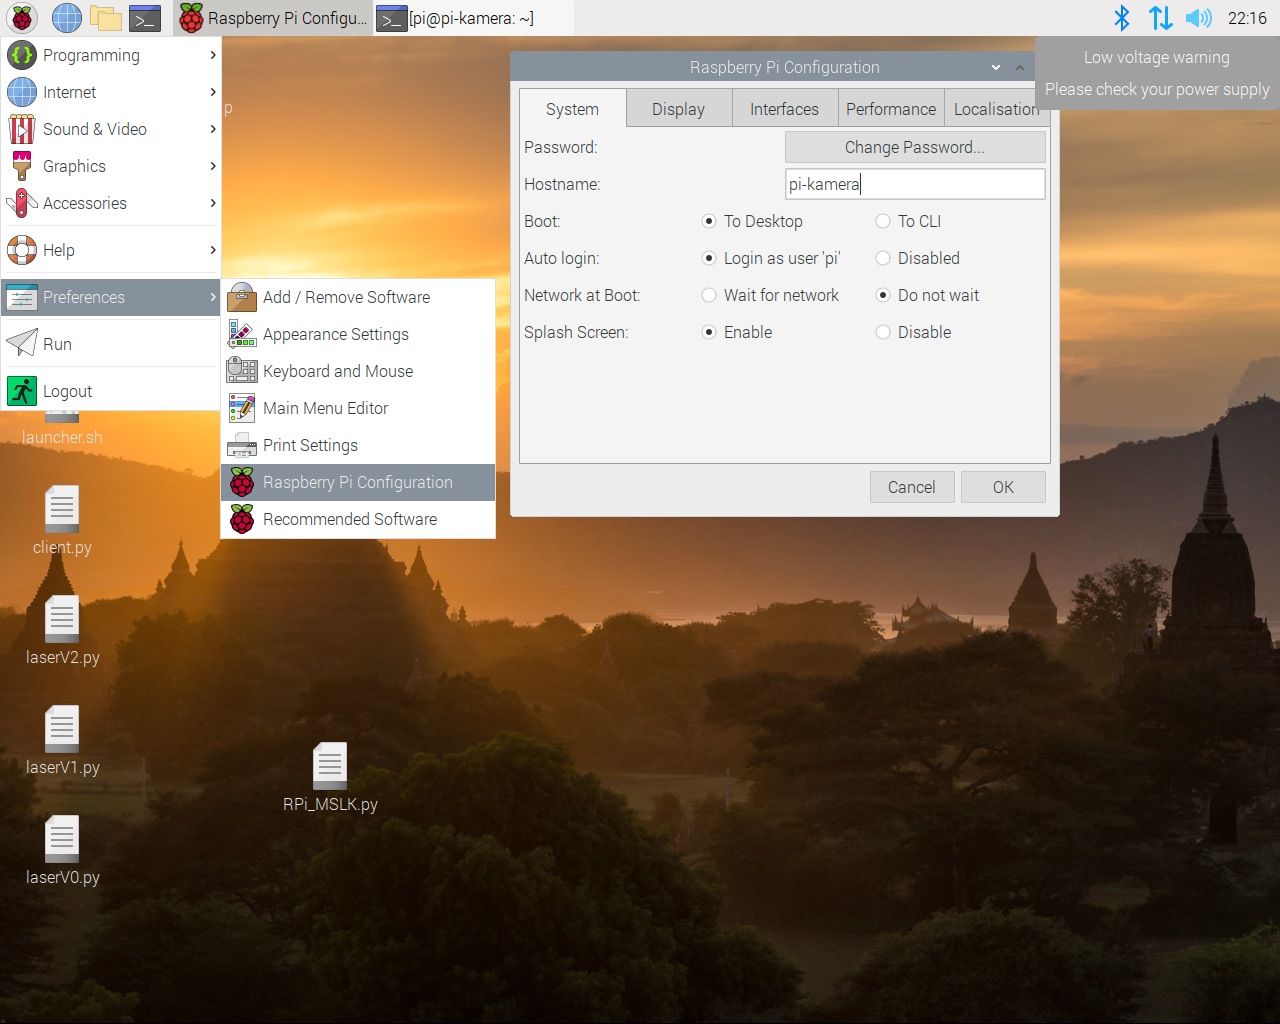
\includegraphics[width=\linewidth]{slike/pi1.png}
    \caption{Nastavlanje RPi.}
    \label{fig:pi_nast}
\end{figure}

\section{PC}
Iz \href{https://github.com/nekajcasa/MSLK}{githuba} je potrebno potegniti in shraniti v isto mapo:
\begin{itemize}
    \item gui.py,
    \item MSLK.py,
    \item celotno mapo files.
\end{itemize}

\section{Laser in krmilna glava}
Na laser se pritrdi krmilno glavo, ki se jo poveže na AO kartico (slika \ref{fig:ao}). 

\begin{figure}[H]
    \centering
    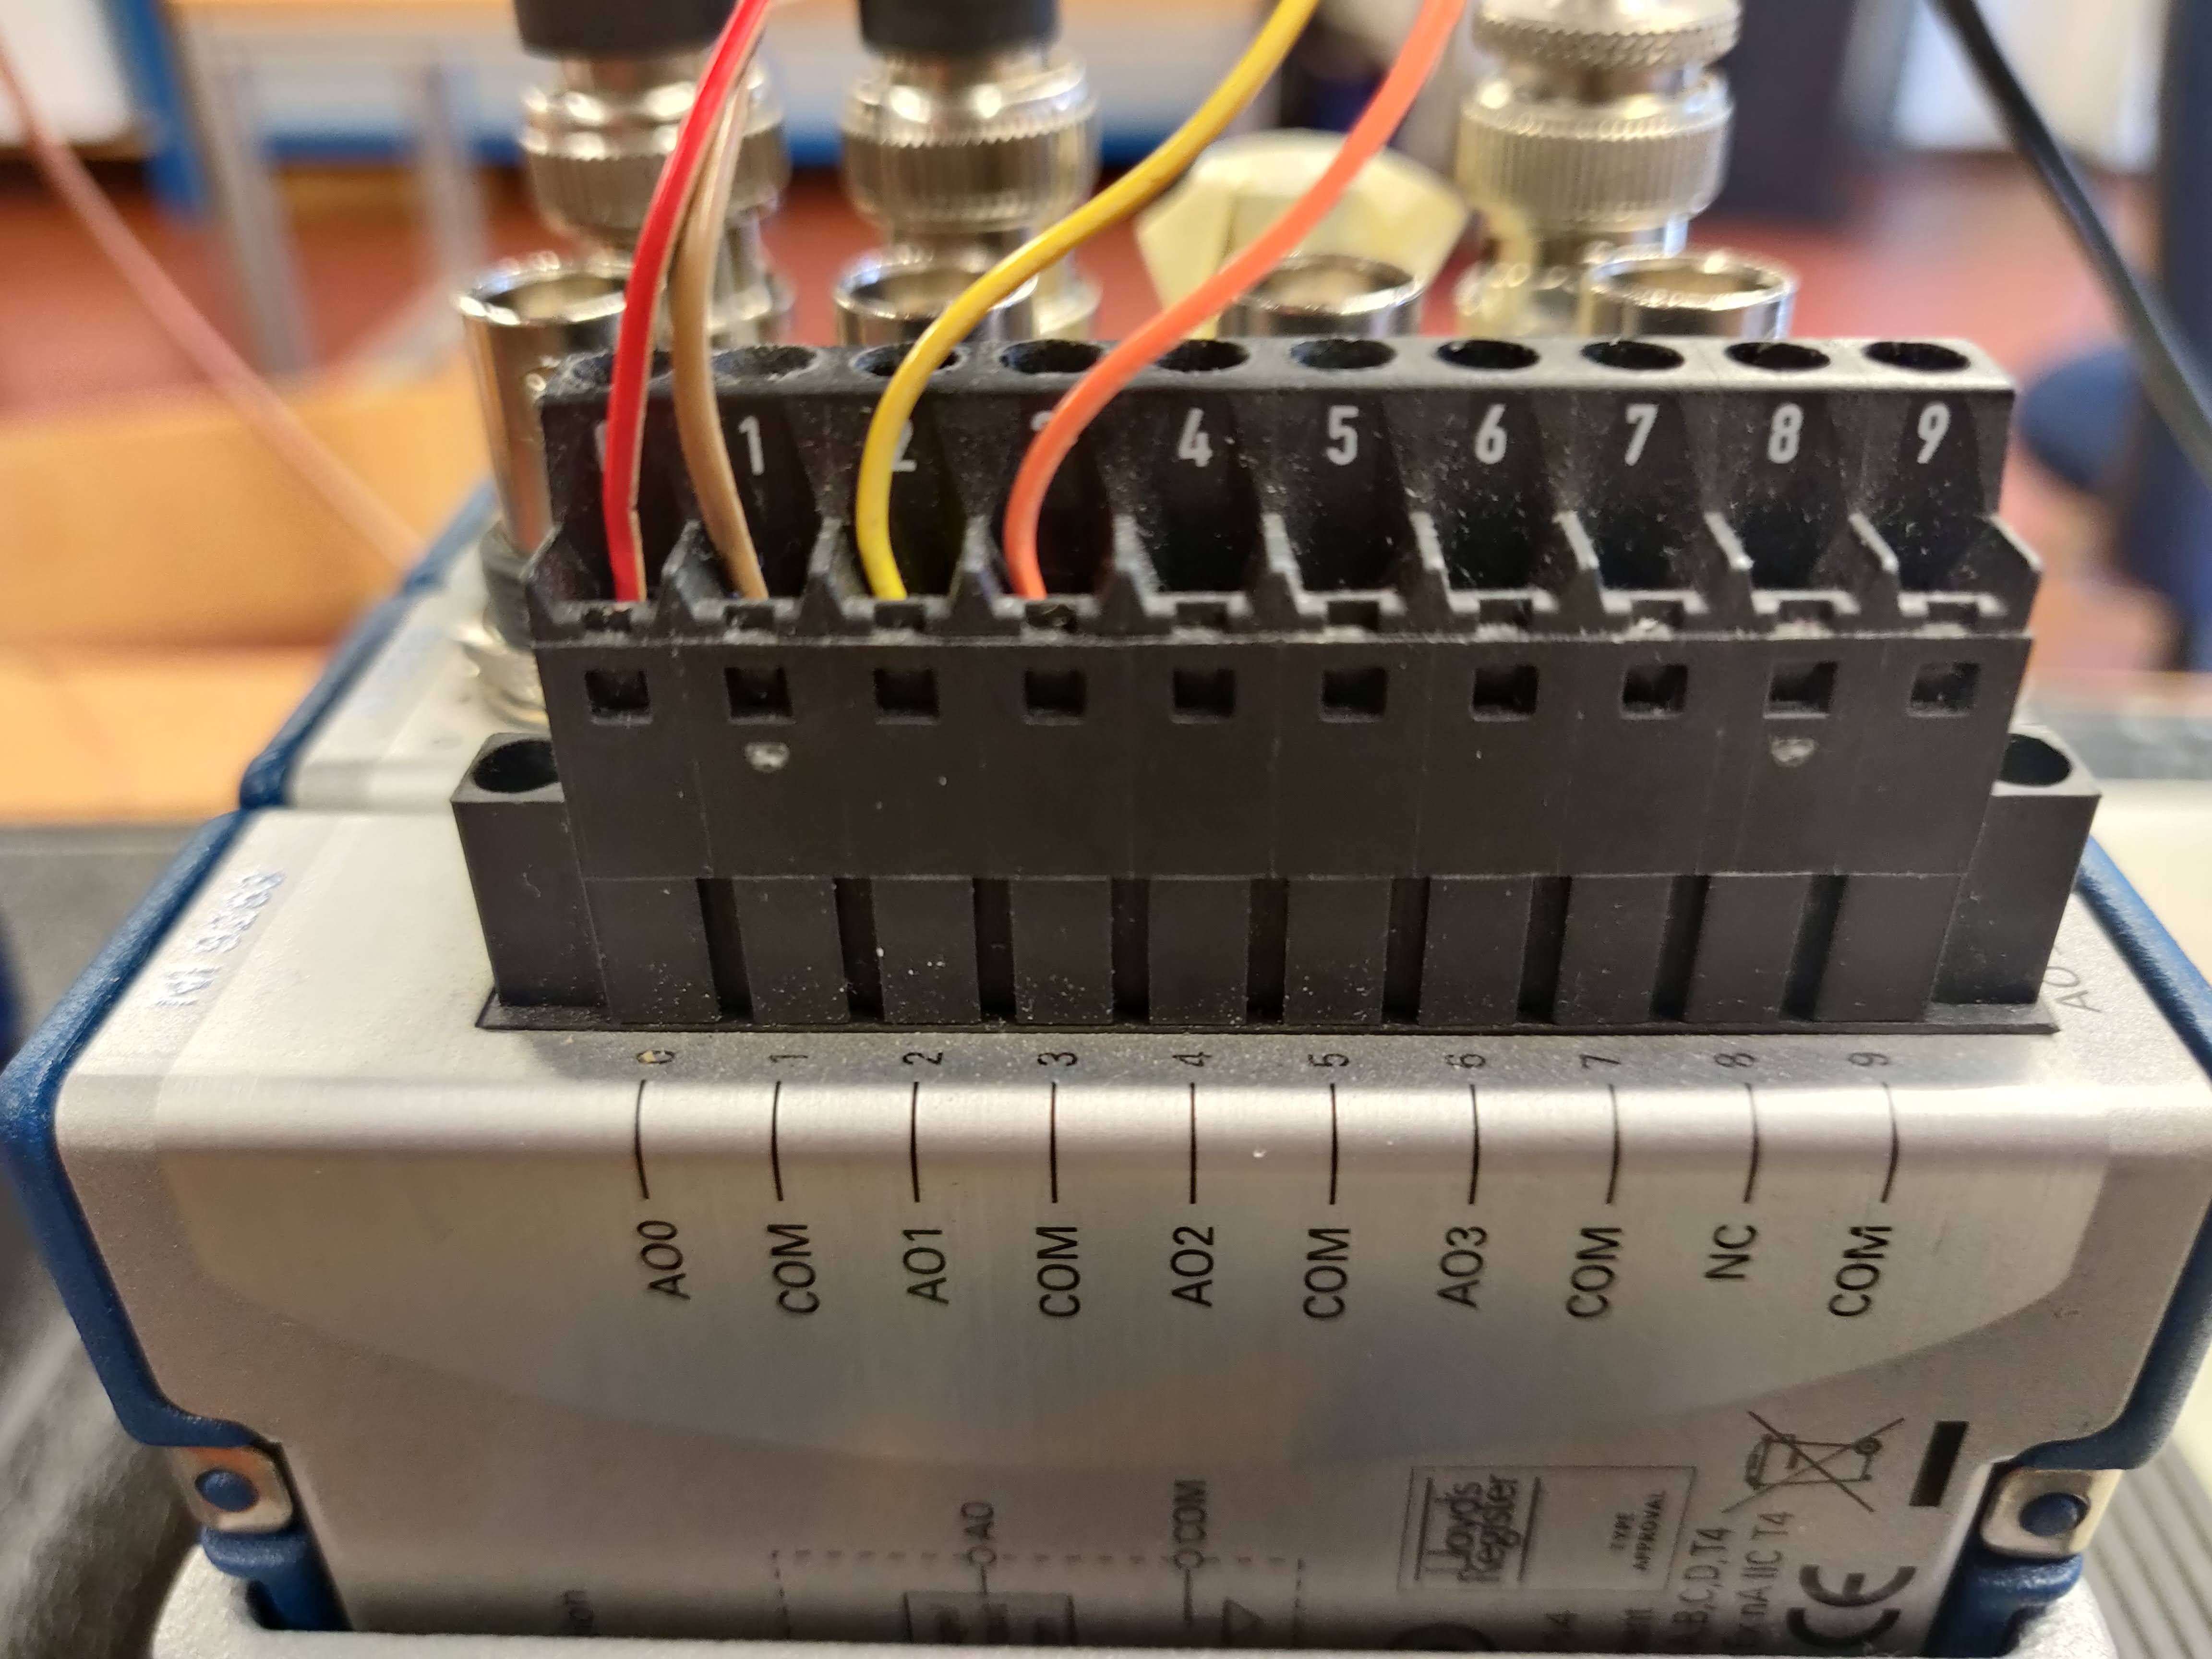
\includegraphics[width=.75\linewidth]{slike/povezava_na_ao.jpg}
    \caption{Povezava krmilne glave na AO.}
    \label{fig:ao}
\end{figure}
Napajamo jo preko napajalnika v zaporedni vezavi s 15V, kakor je prikazano na sliki \ref{fig:napajanje_krmilne_glave}.
\begin{figure}[H]
    \centering
    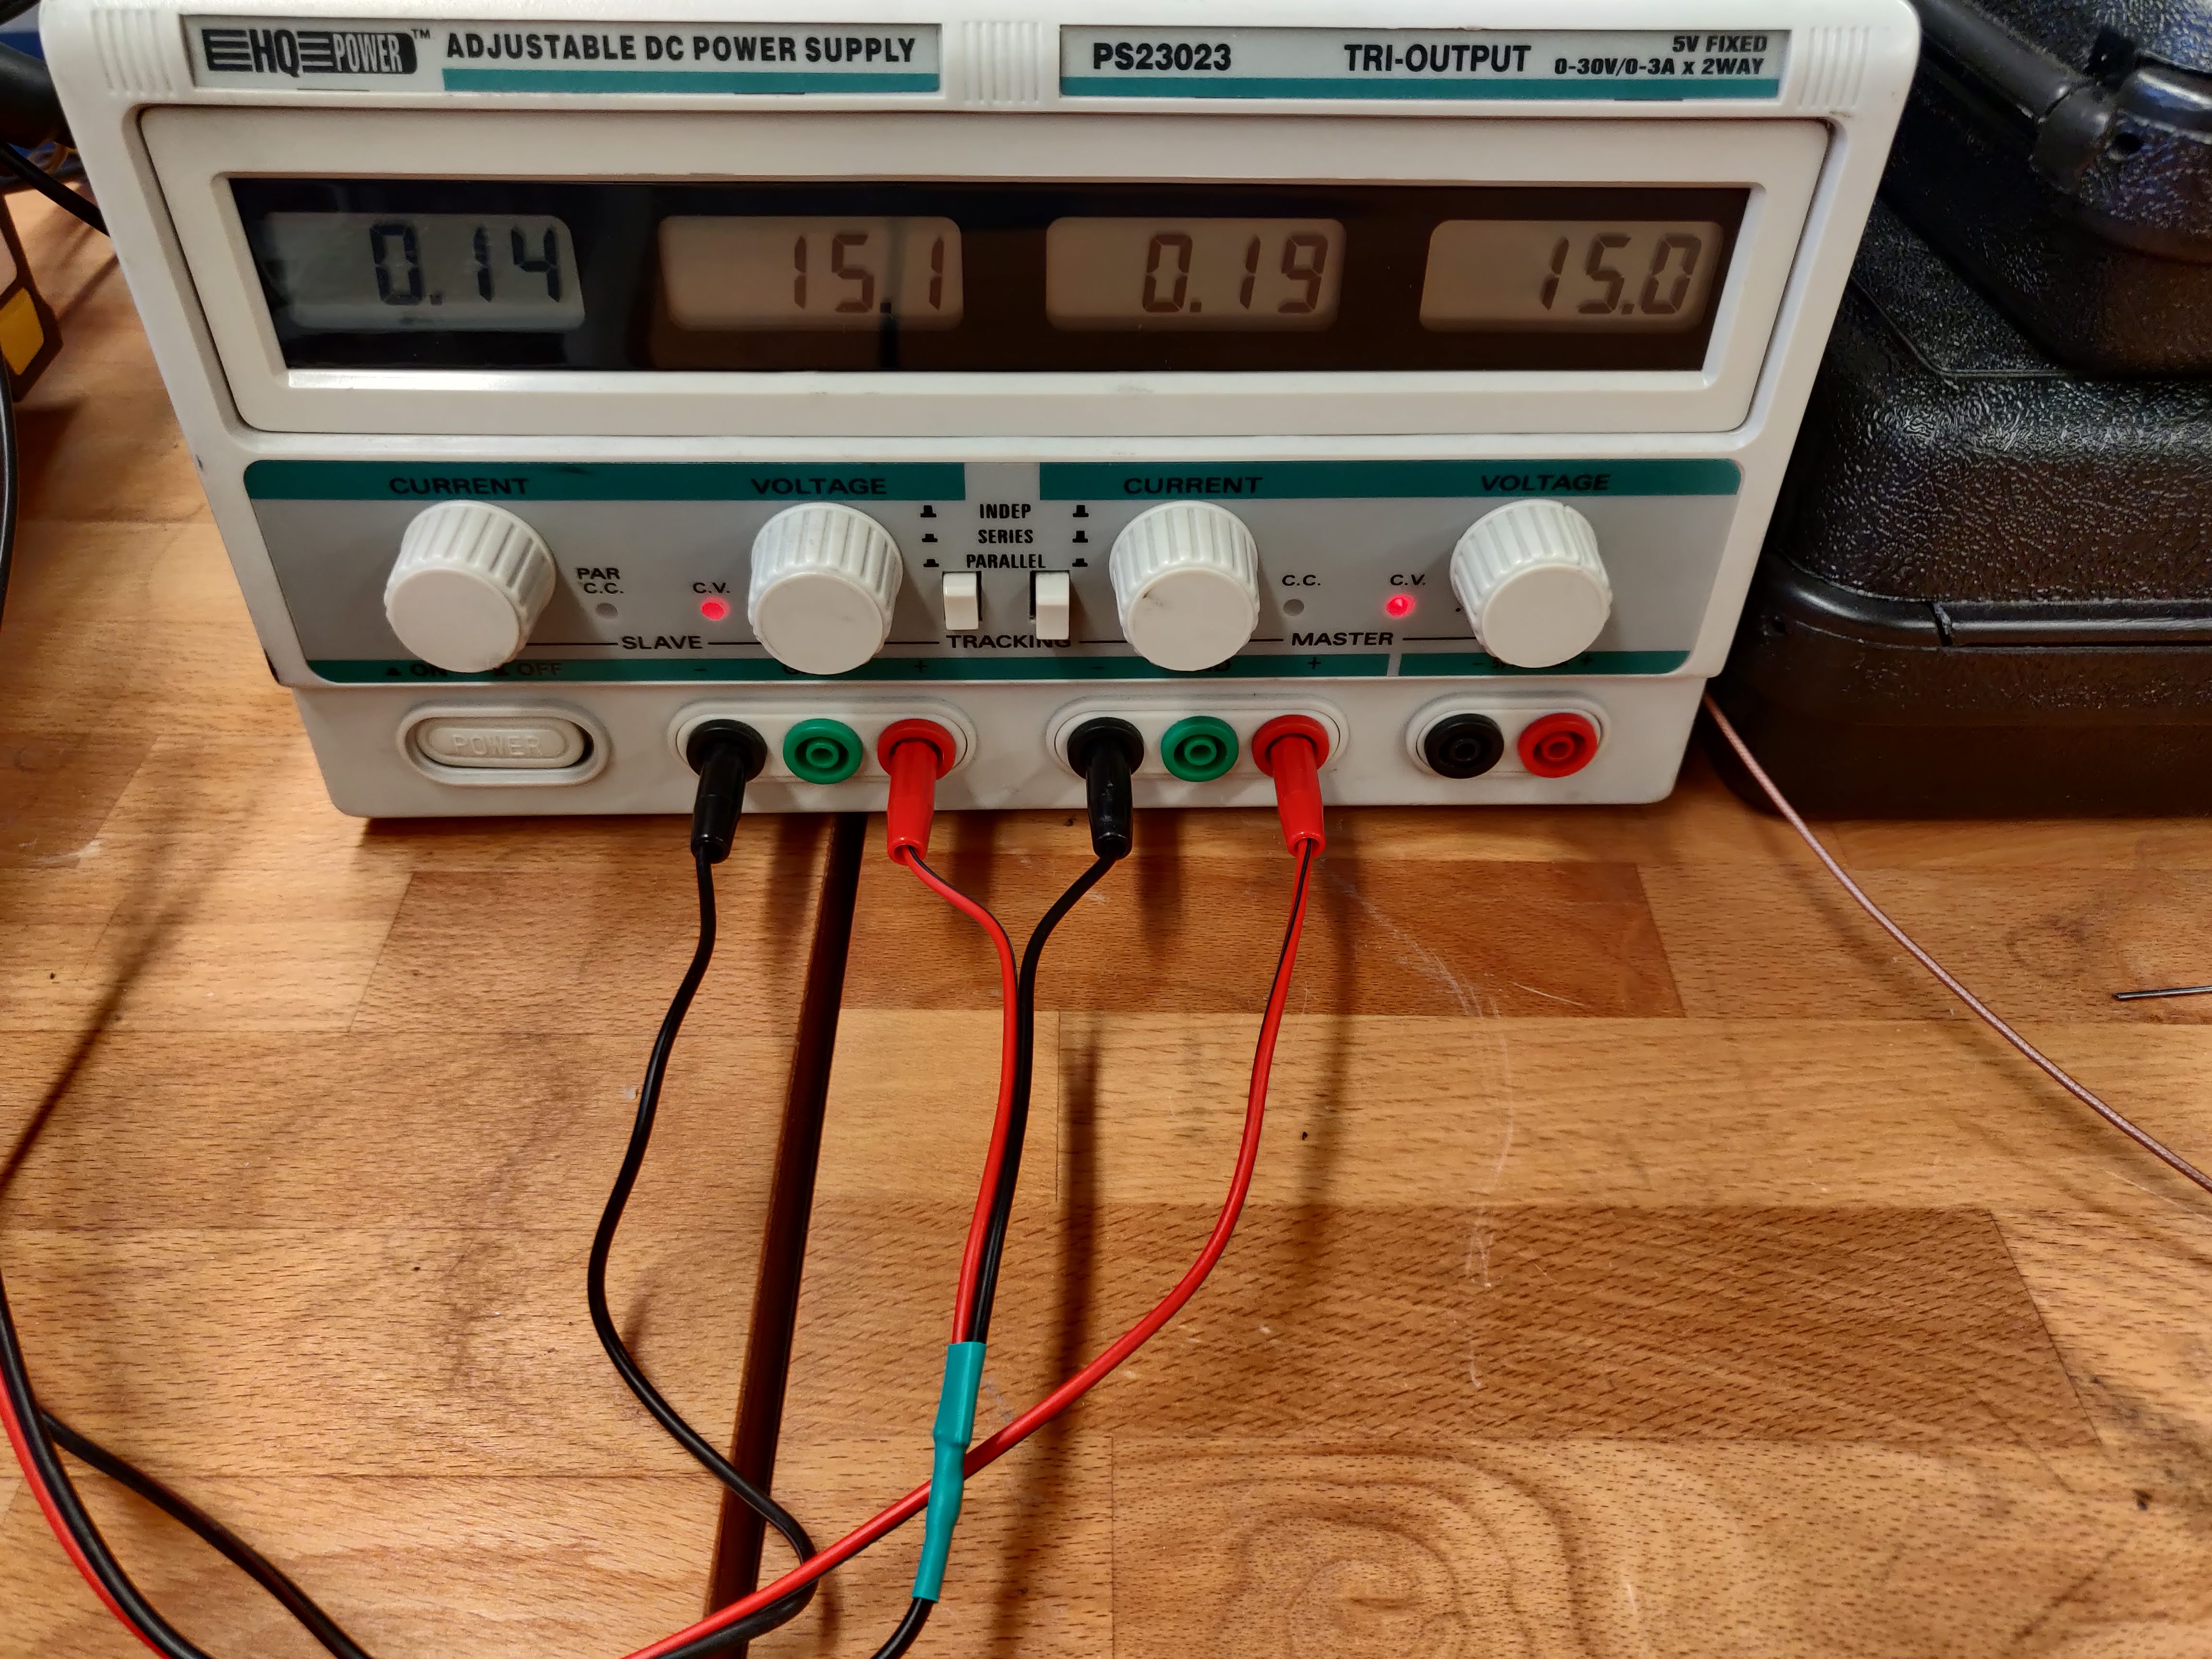
\includegraphics[width=0.75\linewidth]{slike/napajanje_glave.jpg}
    \caption{Napajanje krmilne glave.}
    \label{fig:napajanje_krmilne_glave}
\end{figure}